% !TeX root =./ClassicalElectrodynamics.tex

% chktex-file 1

%========================================================================================================
%
%									      Протоколи
%
%========================================================================================================


% ============ НН ФТІ ==========
\newcommand\IPTNo{13}            % Номер протокола затвердження методичною комісією НН ФТІ
\newcommand\IPTDate{26.10.2026}  % Дата протокола затвердження методичною комісією НН ФТІ

% ============ КПІ =============
\newcommand\KPINo{X}             % Номер протокола надання грифу КПІ
\newcommand\KPIDate{XX.XX.2026}  % Дата протокола надання грифу КПІ

%========================================================================================================
%
%									      Палітурка
%
%========================================================================================================

\newcommand{\CoverPage}{
	\begin{alwayssingle}
		\begin{center}
			\begin{flushright}\bfseries\sffamily
				\MakeUppercase{Міністерство освіти і науки України}\\
				КПІ ім. Ігоря Сікорського\\
			\end{flushright}
			\begin{tcolorbox}[titlepagestyle,
					toprule=0.10cm,
					bottomrule=0.10cm,
					overlay={%
							\node (picture) at ([xshift=4cm]frame.west) {
\includegraphics[width=3.5cm]{logo/logo_IPT}};
						}
				]%
				\begin{flushright}
					\large\bfseries\color{white}Навчально-науковий\\ фізико-технічний інститут
				\end{flushright}
			\end{tcolorbox}
			\vspace*{-2em}
			\begin{Large}\color{themecolordark!90!black}
				\begin{alignat*}{3}
					\vect{\nabla} & \times  &  & \Efield &  & = -\dfrac{1}{c}\dfrac{\partial\Bfield}{\partial t}                         \\
					\vect{\nabla} & \,\cdot &  & \Bfield &  & = 0                                                                        \\
					\vect{\nabla} & \,\cdot &  & \Dfield &  & = 4\pi\rho                                                                 \\
					\vect{\nabla} & \times  &  & \Hfield &  & = \dfrac{4\pi}{c} \vect{j}+\dfrac{1}{c}\dfrac{\partial\Dfield}{\partial t}
				\end{alignat*}
			\end{Large}
			\vspace*{2em}
			\begin{tcolorbox}[
					titlepagestyle,
					toprule=0.15cm,
					bottomrule=0.15cm,
					top=1.3cm,
					bottom=0.7cm,
					overlay={%
							\node[%
								fill=white,
								rounded corners = 15pt,
								draw=themecolorlight,
								line width=0.15cm,
								inner sep=0pt,
								text width=17cm,
								minimum height=2cm,
								align=center,
								%anchor=east,
								font=\sffamily\bfseries\large
							] (title) at (frame.north) {С.~М. Пономаренко
							};
						}
				]
				\centering
				\Huge\sffamily\bfseries\textcolor{white}{\realtitle}\\
				\huge\sffamily\bfseries\textcolor{white}{\subtitle}
			\end{tcolorbox}
			\vfill
			% Адаптовано з MaxwellEqns.tex (слайд "Стаціонарні поля")
\begin{minipage}[t]{0.3\linewidth}\centering
	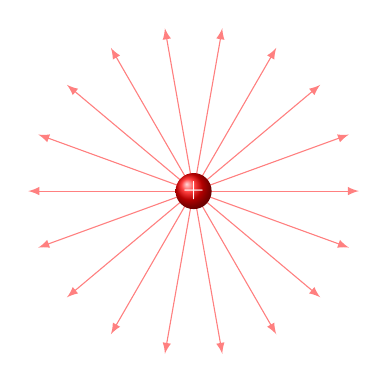
\begin{tikzpicture}[>=latex, scale=1]
		\foreach \i in {20,40,...,360}
			{
				\draw[->, red!50] (0,0)  ++(\i:0.1) -- ++(\i:2);
			}
		\node[circle, inner sep=1pt, ball color=red, text=white] at (0, 0) {$+$};
	\end{tikzpicture}
\end{minipage}
\begin{minipage}[t]{0.3\linewidth}\centering
	\begin{tikzpicture}[>=latex, scale=1]
		\draw [in=-105, out=75, looseness=1.25, line width=0.1cm, gray!50] (-1, -1) coordinate (A)
		to (1, 1.5) coordinate (B);
		\draw[fill=gray!50, ultra thin, rotate around={-10:(B)}] (B) circle(0.05 and 0.015);
		\draw[fill=gray!50, ultra thin, rotate around={-10:(A)}] (A) circle(0.05 and 0.015);
		\draw[thin, blue, rotate around={-15:(-0.25:0)}, arrowpos={0.85}{2pt}{4pt}] (-0.25, 0)
		circle(0.5 and 0.15);
		\draw[thin, blue, rotate around={-15:(-0.25:0)}, arrowpos={0.85}{2pt}{4pt}] (-0.25, 0)
		circle(2 and 0.7);
		\draw[thin, blue, rotate around={-15:(-0.25:0)}, arrowpos={0.85}{2pt}{4pt}] (-0.25, 0)
		circle(1 and 0.3);
		\begin{scope}
			\clip (-1,0) rectangle (1,1);
			\draw [in=-105, out=75, looseness=1.25, line width=0.1cm, gray!50] (A) to (B) ;
		\end{scope}
		\draw [in=-105, out=75, looseness=1.25, gray, arrowpos={0.85}{2pt}{4pt}] (-1, -1)
		coordinate (A) to (1, 1.5) coordinate (B);
	\end{tikzpicture}
\end{minipage}
\begin{minipage}[t]{0.3\linewidth}\centering
\begin{tikzpicture}[rotate=90, scale=1, >=latex, midarrow/.style={%
				postaction={ decorate,
						decoration={ markings, mark=at position .7 with {\arrow{latex}}}}}]
	\begin{scope}[xshift=0.3cm]
		\draw[arrowpos={0.5}{2pt}{4pt}, red] (1.1,0) [partial ellipse=360:0:0.15 and 0.5];
		\draw[arrowpos={0.5}{2pt}{4pt}, red] (1.1,0) [partial ellipse=360:0:0.3 and 1];
		\draw[arrowpos={0.5}{2pt}{4pt}, red] (1.1,0) [partial ellipse=360:0:0.6 and 2] node[pos=0.5,
		below] {$\Efield$};
	\end{scope}
	\foreach \y in {-3,...,3}{
			\draw[blue, midarrow] plot[domain=1:3] (\x, 0.2*\y+0.05*\y*\x^2);
		}
	\node[blue, font=\small] at (3.5, 0) {$\frac{\partial\Bfield}{\partial t}>0$};
\end{tikzpicture}
\end{minipage}


			\vfill
			\begin{tcolorbox}[titlepagestyle,
					toprule=0.10cm,
					bottomrule=0.10cm]
				\begin{center}\color{white}\bfseries\normalsize
					\MakeUppercase{Київ~\the\year} \\
					%					КПІ ім. Ігоря Сікорського \\
					%					\the\year
				\end{center}
			\end{tcolorbox}
		\end{center}
		\clearpage
	\end{alwayssingle}
	\setcounter{page}{1}
}


%========================================================================================================
%
%									      Титульна сторінка
%
%========================================================================================================

\renewcommand\maketitle{
	\begin{alwayssingle}
		\begin{center}
			\MakeUppercase{Міністерство освіти і науки України}

			\bigskip
			\MakeUppercase{Національний технічний університет України}\\
			<<КИЇВСЬКИЙ ПОЛІТЕХНІЧНИЙ ІНСТИТУТ \\ імені ІГОРЯ СІКОРСЬКОГО>>
			\vspace*{100pt}

			{\large С.~М.~Пономаренко
			}
			\vspace*{50pt}

			{\Huge\sffamily\bfseries\realtitle}\\[1em]
			{\huge\sffamily\bfseries\subtitle}

			\vspace*{50pt}
			\begin{center}\itshape
				Затверджено Вченою радою КПІ ім. Ігоря Сікорського як підручник для
				здобувачів ступеня бакалавра за спеціальностями E6 Прикладна фізика та наноматеріали.
			\end{center}
			\vfill
			%                 \textcolor{malina}{Видання друге, виправлене та доповнене}
			%                \textcolor{malina}{Версія від~\today, час компіляції \currenttime.}
			\vfill
			\begin{center}
				\MakeUppercase{Київ} \\
				КПІ ім. Ігоря Сікорського \\
				\the\year
			\end{center}
		\end{center}
		\clearpage
	\end{alwayssingle}
}


%========================================================================================================
%
%									      Друга сторінка
%
%========================================================================================================
\newcommand\makeinfopage{
	\begin{alwayssingle}
		\noindent%
		\begin{minipage}[t]{0.5\textwidth}
			\begin{flushleft}
				УДК  537(075.8)\\
				ББК  22.31я73\\
				П 563
			\end{flushleft}
		\end{minipage}


		\bigskip\noindent%
		\begin{minipage}[t]{0.25\linewidth}
			\begin{flushleft}
				Рецензенти:
			\end{flushleft}
		\end{minipage}\hfill
		\begin{minipage}[t]{0.75\linewidth}
			\href{https://staff.lpnu.ua/profile/Ihor.R.Zachek}{І.~Р.~Зачек}, д.ф.-м.н.,
			професор кафедри загальної фізики Інституту прикладної математики та
			фундаментальних наук Національного університету <<Львівська політехніка>>.
			\\[1ex]
			\href{https://esu.com.ua/article-76544}{О.~Я.~Оліх}, д.ф.-м.н., професор,
			завідувач кафедри загальної фізики, фізичного факультету КНУ імені Тараса
			Шевченка.
		\end{minipage}

		\bigskip\noindent%
		\begin{minipage}[t]{0.25\linewidth}
			\begin{flushleft}
				Відповідальний редактор:
			\end{flushleft}
		\end{minipage}\hfill
		\begin{minipage}[t]{0.75\linewidth}
			\href{https://is.ipt.kpi.ua/is/litvinovatv/}{Т.~В.~Литвинова}, к.т.н.,
			доцент, перший заступник директора НН ФТІ КПІ ім. Ігоря Сікорського.
		\end{minipage}

		\vfill

		\begin{center}\itshape\small
			Гриф надано Вченою радою КПІ ім. Ігоря Сікорського (протокол №~\KPINo~від \KPIDate~р.) за поданням Вченої ради Навчально-наукового Фізико-технічного інституту (протокол №~\IPTNo~від \IPTDate~р.)
		\end{center}
		\vfill
		% 		\begin{center}
		% 			\ifelectronic Електронне мережне навчальне видання \fi
		% 			%\par {Версія від~\href{http://www.istpravda.com.ua/dates}{\today}} \par\else \par  \fi
		% 		\end{center}
		% 		\begin{center}
		% 			\href{https://apd.ipt.kpi.ua/kafedra/stuff/ponomarenko}{\itshape Пономаренко Сергій
		% 			Миколайович}, к.ф.-м.н., доцент
		% 		\end{center}
		% %			\vspace*{1em}%
		% 		\begin{center}\bfseries
		% 			\LARGE\sffamily\realtitle \\
		% 			\Large\sffamily\subtitle
		% 		\end{center}

		% ========================================================
		\noindent
		\phantom{П 563}\hfill%
		\begin{minipage}[t]{0.85\textwidth}\small
			\textbf{Пономаренко С.М.}
		\end{minipage}
		% ========================================================

		\noindent%
		П 563\hfill \begin{minipage}[t]{0.85\textwidth}\small
			\hspace{2em}\realtitle\ [Електронний ресурс] : підруч. для студ. спеціальностей
			E6 <<Прикладна фізика та наноматеріали>> / С.~М. Пономаренко; КПІ ім. Ігоря Сікорського.~--- Електронні
			текстові дані
			(1 файл: 16{,}6~МБ). – Київ: КПІ ім. Ігоря Сікорського, \the\year. ---
			\the\numexpr\getpagerefnumber{LastPages}-1\relax~с.
		\end{minipage}

		%		\noindent%
		%		\begin{flushleft}
		%			\begin{tabular}{lp{0.9\textwidth}}
		%				     & В.~І. Жданов, С.~М. Пономаренко, В.~Б. Долгошей                                                                                                                                                                        \\
		%				Ж 42 & \hspace*{3ex} \realtitle : \subtitle{} [Електронний ресурс] : навчальний посібник / %
		%				В.~І. Жданов, %
		%				С.~М. Пономаренко%,
		%				В.~Б. Долгошей %
		%				--- К.:~КПІ ім. Ігоря Сікорського, \the\year. --~\the\numexpr\getpagerefnumber{LastPage}-1\relax~с. -- Бібліогр.: с.~\pageref{BibPage}\relax. \ifelectronic\relax\else-- 80~прим.\fi
		%			\end{tabular}
		%		\end{flushleft}
		\vfill


		Для студентів фізико-технічного інституту КПІ ім. Ігоря Сікорського, які навчаються за спеціальностями E6~Прикладна фізика та наноматеріали.

		\vfill

		\begin{center}\scriptsize
			Реєстр. № П ХХ/ХХ-ХХХ. Обсяг Х,Х авт. арк.\\
			Національний технічний університет України \\
			«Київський політехнічний інститут імені Ігоря Сікорського»\\
			проспект Берестейський, 37, м. Київ, 03056\\
			\url{https://kpi.ua}\\
			Свідоцтво про внесення до Державного реєстру видавців, виготовлювачів \\
			і розповсюджувачів видавничої продукції ДК № 5354 від 25.05.2017 р.
		\end{center}

		\vfill
		
		\begin{flushright}
			\begin{minipage}[t]{0.6\linewidth}\small
				\textcopyright{} С.~М. Пономаренко, \the\year\,р. \\
				\textcopyright{}  КПІ ім. Ігоря Сікорського (НН ФТІ), \the\year~р.
			\end{minipage}
		\end{flushright}
		\newpage%
	\end{alwayssingle}
}

%%%%%%%%%%%%%%%%%%%%%%%%%%%%%%%%%%%%%%%%%%%%%%%%%%%%%%%%%%%%%%%%%%%%%%%%%%%%
%%                                                                        %%
%%                              Last Page                                 %%
%%                                                                        %%
%%%%%%%%%%%%%%%%%%%%%%%%%%%%%%%%%%%%%%%%%%%%%%%%%%%%%%%%%%%%%%%%%%%%%%%%%%%%
\newcommand{\makelastpage}{%
	\clearpage%
	\thispagestyle{empty}%
	\vspace*{0.4\textheight}
	\begin{center}
		\textbf{Пономаренко} Сергій Миколайович
	\end{center}

	\begin{center}\bfseries
		\Large\sffamily\realtitle \\
		\large\sffamily\subtitle
	\end{center}

	\begin{center}\itshape
		Комп'ютерне верстання в системі \LaTeXe{} С.\ М. Пономаренко
	\end{center}

	\vspace*{1em}
	\begin{center}\small
		Національний технічний університет України \\
		<<Київський політехнічний інститут імені Ігоря Сікорського>> \\
		Свідоцтво про державну реєстрацію: серія ДК № 5354 від 25.05.2017 р.\\
		просп. Берестейський, 37, м. Київ, 03056
	\end{center}

	%\vfill
	%
	%\begin{center}
	%    Видавництво <<Політехніка>> \kpishort \\
	%    вул. Політехнічна, 14, корп. 15 \\
	%    м. Київ, 03056 \\
	%    Тел. (044) 204-81-78
	%\end{center}
}


